%%%%%%%%%%%%%%%%%%%%%%%%%%%%%%%%%%%%%%%%%%%%%%%%%%%%%%%%%%%%%%%%%%%%%%%%%%%%%%%%
\documentclass[letterpaper, 10pt, journal, twoside]{IEEEtran}
\pdfobjcompresslevel=0
\pdfminorversion=4
\usepackage{amsmath}
\usepackage[colorlinks=true, linkcolor=blue, urlcolor=blue, citecolor=blue]{hyperref}
\usepackage{cleveref}
\usepackage[ruled,vlined,linesnumbered]{algorithm2e}
\usepackage{graphicx}
\usepackage{booktabs}
\usepackage{multirow}
\usepackage{multicol}
\usepackage{subcaption}
\usepackage{enumitem}
\usepackage{amssymb}
\usepackage{mathpartir}
\usepackage{makecell}
\usepackage{bm}
\usepackage{xspace}
\usepackage{pifont}
\usepackage{nicefrac}
\usepackage{stfloats}
\usepackage{rotating}

\let\llncssubparagraph\subparagraph
\let\subparagraph\paragraph
\usepackage[compact]{titlesec}
\let\subparagraph\llncssubparagraph
\titlespacing{\section}{0pt}{4pt}{1pt}
\titlespacing{\subsection}{0pt}{3pt}{1pt}
\titlespacing{\subsubsection}{0pt}{2pt}{1pt}

\setlength{\abovedisplayskip}{4pt}
\setlength{\belowdisplayskip}{4pt}

% Float placement tuning — allow more floats per page, reduce excessive whitespace
\renewcommand{\topfraction}{0.90}
\renewcommand{\textfraction}{0.07}
\renewcommand{\floatpagefraction}{0.85}
\setcounter{topnumber}{4}
\setcounter{totalnumber}{8}
\setlength{\textfloatsep}{8pt plus 2pt minus 2pt}
\setlength{\floatsep}{6pt plus 2pt minus 2pt}

\newcommand{\fref}[1]{Fig.~\ref{#1}}
\newcommand{\sref}[1]{Section~\ref{#1}}
\newcommand{\tref}[1]{Table~\ref{#1}}
\newcommand{\myparagraph}[1]{\noindent\textbf{#1}~}
\newcommand{\eref}[1]{(\ref{#1})}
\newcommand{\method}{LLM-Flax\xspace}
\newcommand{\baseline}{Flax\xspace}
\newcommand{\fullmethod}{Full LLM-Flax\xspace}

\title{\LARGE \bf
LLM-Flax : Toward Generalizable Robotic Task Planning via Neuro-Symbolic Approaches with Large Language Models
}

\author{Seongmin Kim$^{1}$, Daegyu Lee$^{2*}$%
% \thanks{Manuscript submitted: April, 2026.}
\thanks{$^{1}$Seongmin Kim is with the Department of Physical AI Engineering, Jeonbuk National University(JBNU)}
\thanks{$^{2}$Daegyu Lee is with Faculty of Department of Advanced Defense Technology and Industry, Jeonbuk National University(JBNU)}
\thanks{$^{*}$Corresponding author}
}

\begin{document}

\maketitle

%%%%%%%%%%%%%%%%%%%%%%%%%%%%%%%%%%%%%%%%%%%%%%%%%%%%%%%%%%%%%%%%%%%%%%%%%%%%%%%%
\begin{abstract}
Deploying a neuro-symbolic task planner on a new domain today requires a domain expert to author relaxation and complementary rules and hundreds of training problems to supervise a Graph Neural Network (GNN) object scorer.
We propose \method, a three-stage framework that targets all three costs using a locally hosted LLM given only a PDDL domain file: Stage~1 generates relaxation and complementary rules via structured prompting with validation and self-correction; Stage~2 adds LLM-guided failure recovery under a feasibility-gated budget policy; and Stage~3 replaces the trained GNN with zero-shot LLM object scoring.
We evaluate Stage~1 on eight MazeNamo benchmarks plus two further PDDL domains (DifficultLogistics, SokomindPlus) to probe generalization beyond a single domain.
On MazeNamo, \method achieves average SR~0.941 versus Manual's 0.912 ($+0.029$), matching or exceeding Manual on every benchmark; a controlled ablation confirms this is driven by rule content, not rule count.
Cross-domain, \method matches or exceeds Manual on both further domains: on SokomindPlus directly, and on DifficultLogistics after we identify and fix a shared planner-loop bug---invisible on MazeNamo/SokomindPlus but exposed by DifficultLogistics's global connectivity constraints---that had caused both rule sources to fail outright.
Stage~3 shows partial feasibility (SR~0.533 on $12{\times}12$ Hard, no training data) but collapses at larger scale (SR~0.000 on $15{\times}15$ Hard); instrumenting the LLM's output shows the cause is not a context-window limit but an output-generation failure---the model stops early, leaving 70--99\% of objects silently unscored---a more specific and tractable target than previously characterized.
\end{abstract}

\begin{IEEEkeywords}
Task Planning, Large Language Models, Neuro-Symbolic AI, PDDL, Zero-Shot Generalization
\end{IEEEkeywords}

%%%%%%%%%%%%%%%%%%%%%%%%%%%%%%%%%%%%%%%%%%%%%%%%%%%%%%%%%%%%%%%%%%%%%%%%%%%%%%%%
\section{Introduction}
\IEEEPARstart{T}{ask} planning in complex, object-rich environments requires long-horizon reasoning over large state spaces, making classical symbolic planners computationally expensive~\cite{helmert2006fast,edelkamp2004pddl2}.
Neuro-symbolic methods address this scalability challenge by using neural networks to identify a small subset of relevant objects, reducing the grounded planning problem size before invoking a symbolic solver~\cite{silver2021planning,chen2024graph}.

\begin{figure*}[t]
  \centering
  
\includegraphics[width=0.85\textwidth]{figures/teaser.pdf}
  \caption{Overview of \method. Given only a PDDL domain file, Stage~1 automatically generates relaxation and complementary rules; Stage~2 provides budget-aware LLM failure recovery; and Stage~3 replaces the domain-trained GNN with zero-shot LLM object scoring. Together, the full \fullmethod system deploys on a new domain with no manual engineering.}
  \label{fig:teaser}
\end{figure*}

A representative framework of this kind, Flax~\cite{du2026fast}, combines a Graph Neural Network (GNN) for object importance prediction with domain-specific symbolic rules in two roles: (1) \emph{relaxation rules} that remove non-essential objects to produce a simplified, easier-to-solve version of the problem, and (2) \emph{complementary rules} that restore object pairs connected by spatial or structural constraints.
Together these components enable fast, reliable planning even on expert-level maze tasks where classical planners time out.

Despite strong empirical performance, deploying such a planner on a new domain requires three distinct forms of manual labor:
\textbf{(1)} an expert must author relaxation rules encoding which objects are removable and under what conditions;
\textbf{(2)} an expert must author complementary rules encoding which object pairs must appear together; and
\textbf{(3)} hundreds of training problems must be solved offline to train the GNN scorer.
Together, these requirements make it impractical to apply the system to a new domain without significant engineering investment.

Recent rapid progress in large language models (LLMs) opens a path to eliminating all three bottlenecks.
Modern LLMs demonstrate strong capabilities in structured reasoning, formal language understanding, and code generation~\cite{brown2020language,wei2022chain}.
We hypothesize that an LLM, given only a PDDL domain file, can automatically infer predicate semantics, generate valid planning rules, recover from plan failures with semantic guidance, and score object importance zero-shot---replacing every source of manual domain knowledge.

In this paper we present \method, a three-stage framework realizing this vision:
\begin{itemize}[noitemsep,topsep=2pt]
    \item \textbf{Stage 1 --- LLM Rule Generation:} Structured prompting with format validation and self-correction generates relaxation and complementary rules directly from the PDDL domain file.
    \item \textbf{Stage 2 --- LLM Failure Recovery:} When GNN-guided planning times out, an LLM analyzes the current state and goal to identify missing objects; a budget-aware policy ensures that API latency cost is explicitly reserved before the call, preventing the downstream relaxation step from being starved.
    \item \textbf{Stage 3 --- LLM Zero-Shot Object Scoring:} An LLM scores object importance from the PDDL state and goal without any training data, replacing the domain-trained GNN entirely.
\end{itemize}
The combined \fullmethod system requires only a PDDL domain file to deploy on a new domain.
We evaluate all three stages on the MazeNamo benchmark and report their contributions and limitations.


\section{Related Work}
\label{sec:related}

\subsection{Neuro-Symbolic Task Planning}
Classical symbolic planners such as Fast Downward~\cite{helmert2006fast} and FF~\cite{hoffmann2001ff} provide completeness guarantees but scale poorly with problem size.
STRIPS~\cite{fikes1971strips} established the foundational formalism, while PDDLStream~\cite{garrett2020pddlstream} extended it to continuous domains via blackbox samplers.
Neuro-symbolic approaches address scalability by coupling neural components with symbolic solvers.
PLOI~\cite{silver2021planning} introduced GNN-based object filtering, reducing the grounded state space while preserving validity through iterative threshold relaxation.
Subsequent work explored neuro-symbolic skills~\cite{silver2022neurosymbolic}, relational transition models~\cite{chitnis2022learning}, predicate invention~\cite{silver2023predicate}, and efficient abstract planning models~\cite{kumar2023learning}.
LogiCity~\cite{li2024logicity} further advances neuro-symbolic AI through large-scale abstract urban simulation.

\textbf{The system we directly extend} is Flax~\cite{du2026fast}, which combines a GNN object scorer with hand-crafted relaxation and complementary rules to achieve fast, reliable planning on object-rich PDDL instances.
\method preserves the Flax planning loop entirely and contributes three stages of automation on top of it, eliminating all manual domain engineering.

\subsection{LLMs for Planning and Formal Reasoning}
LLMs have been applied to task planning in multiple ways, which fall into two broad categories relative to our approach.
The first uses the LLM \emph{as the planner or translator}: SayCan~\cite{ahn2022can} grounds LLM outputs directly in robot affordances, LLM+P~\cite{liu2023llm+} uses an LLM to translate natural-language tasks into PDDL problem files for an external solver, and PDDLego~\cite{zhang2023pddl} and~\cite{guan2023leveraging} use LLMs to author or repair whole PDDL domains/problems from scratch.
In each case the LLM's output is consumed once, per task instance, by a downstream solver or policy.
The second category, which includes Tree-of-Thoughts~\cite{yao2023tree} and chain-of-thought prompting~\cite{wei2022chain}, uses the LLM itself as the reasoning engine that searches over or decomposes the problem.
\method belongs to neither category: the LLM is queried \emph{offline, once per domain} (not per task instance) to produce a small, reusable, structured \emph{rule configuration} (relaxation and complementary rules, \sref{sec:format}) that configures an otherwise-unmodified symbolic planner, and separately to provide bounded, budget-gated runtime assistance (Stage~2 failure recovery) to that same unmodified planning loop.
The LLM never proposes a plan, a PDDL problem, or a domain; it only proposes configuration for the existing Flax~\cite{du2026fast} pipeline.
This distinction matters practically: prior LLM-for-planning approaches inherit the LLM's error modes (hallucinated preconditions, invalid grounding) directly into every plan, whereas in \method such errors are caught once, per domain, by the offline validation-and-retry loop (\sref{sec:generation}) before any test-time planning occurs.

\subsection{Automated Knowledge Engineering}
Automated PDDL domain acquisition~\cite{cresswell2013acquiring} and rule learning~\cite{law2019inductive} are classical problems in AI planning.
Our approach differs in that we leverage an LLM's pre-trained world knowledge rather than learning from interaction traces, and we target the specific structured JSON format required by the Flax~\cite{du2026fast} planner rather than full domain synthesis.


\section{Background}
\label{sec:background}

\subsection{PDDL Planning}
A PDDL planning problem $\Pi = \langle \mathcal{D}, \tau \rangle$ consists of a domain $\mathcal{D} = \langle \mathcal{P}, \mathcal{A} \rangle$ defining lifted predicates and actions, and a task instance $\tau = \langle \mathcal{O}, I, G \rangle$ specifying objects, initial state, and goal.
A plan is a sequence of grounded actions mapping $I$ to a state satisfying $G$.

\subsection{Neuro-Symbolic Planning with Rules}
\label{sec:flax_bg}
The baseline planner we extend, Flax~\cite{du2026fast}, operates in three steps during inference:

\myparagraph{Step 1 (GNN Pruning)}
A GNN assigns importance scores $s(o) \in [0,1]$ to each object. Starting from threshold $q = 0.81$ with decay $\gamma = 0.9$, the planner iteratively lowers $q$ and attempts to plan on the pruned object set $\mathcal{O}_1 = \{o \mid s(o) \geq q\}$ until success or timeout.

\myparagraph{Step 2 (Relaxation)}
If Step 1 times out, \emph{relaxation rules} remove certain objects from the full problem to create a simplified ``rough'' version. A rough plan $\mu_r$ is obtained quickly; objects in $\mu_r$ are merged back: $\mathcal{O}_2 = \mathcal{O}_1 \cup \{o \mid o \in \mu_r\}$.

\myparagraph{Step 3 (Complementary Expansion)}
\emph{Complementary rules} restore object pairs connected by structural constraints, yielding $\mathcal{O}_3 = \textsc{Comp}(\mathcal{O}_2)$, on which the final plan is computed.

Both rule types are stored as structured JSON configurations (see \sref{sec:method}) and loaded at runtime.
In the original system, these files are authored manually per domain.


\section{Methodology}
\label{sec:method}

\begin{figure*}[t]
  \centering
  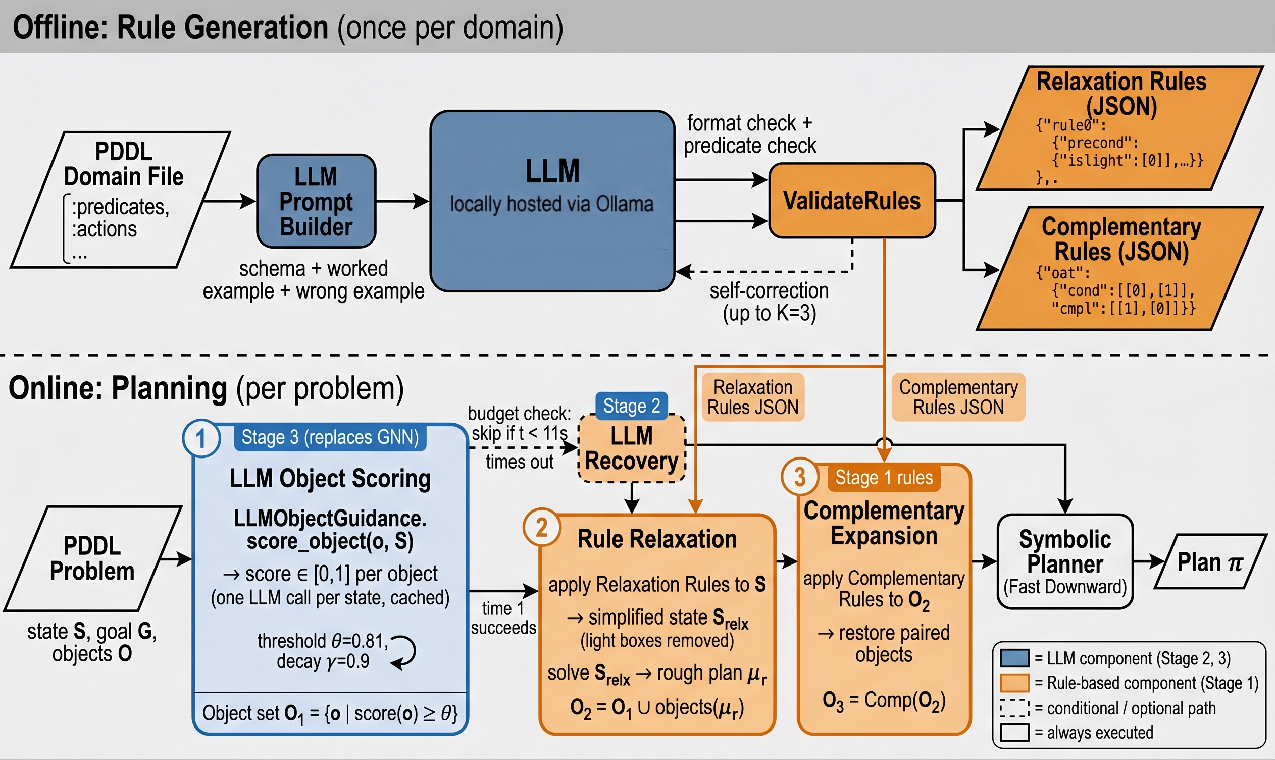
\includegraphics[width=0.85\textwidth]{figures/architecture.pdf}
  \caption{Detailed architecture of \method. \emph{Left}: Stage~1 generates relaxation and complementary rules offline from the PDDL domain file via structured LLM prompting with validation and self-correction. \emph{Center}: At test time, the three-step Flax planning loop (Step~1: threshold-decay pruning; Step~2: relaxation; Step~3: complementary expansion) is shared by all stages. \emph{Right}: Stage~2 inserts a feasibility-gated LLM recovery call between a Step~1 timeout and the Step~2 fallback; Stage~3 replaces the GNN scorer with a zero-shot LLM object scorer. Dashed components require no manual authoring or training data.}
  \label{fig:architecture}
\end{figure*}

\subsection{Rule Format}
\label{sec:format}

\myparagraph{Relaxation rules}
Each rule specifies: (i) \texttt{pre\_compute}—a binary predicate used to look up a related object (e.g., \texttt{oAt} maps an obstacle to its position); (ii) \texttt{precond}—unary predicate(s) identifying removable objects; (iii) \texttt{delete\_objects}—argument index of the object to remove; (iv) \texttt{delete\_effects}—literals to retract; (v) \texttt{add\_effects}—literals to assert after removal.
All values are integer argument indices (0-based).

The manually crafted relaxation rule for MazeNamo reads:
\begin{small}
\begin{verbatim}
{"rule0": {"pre_compute": {"oat":[0,1]},
  "precond": {"islight":[0]},
  "delete_objects": [0],
  "delete_effects": {"islight":[0],
    "ismoveable":[0], "oat":[0,1]},
  "add_effects": {"posempty":[1]}}}
\end{verbatim}
\end{small}

Semantically: \emph{for any light obstacle \texttt{o} at position \texttt{p}, remove \texttt{o} from the problem and mark \texttt{p} as empty.}

\myparagraph{Complementary rules}
Each entry maps a binary predicate name to paired \texttt{cond}/\texttt{cmpl} index lists.
When an object at index \texttt{cond[i]} is included, the object at index \texttt{cmpl[i]} is also included.
The manually crafted complementary rule is simply \texttt{\{"oat": \{"cond":[[0],[1]], "cmpl":[[1],[0]]\}\}}.

\subsection{LLM Rule Generation}
\label{sec:generation}

We use a locally hosted open-source LLM (Gemma3-12B~\cite{gemma3_2025}) served via Ollama with a native REST API.
The LLM is queried twice per domain---once for each rule type---using the following prompting strategy.

\myparagraph{Prompt design}
Each prompt includes: (1) a concise natural-language explanation of the rule type's purpose; (2) the exact JSON schema annotated with field semantics; (3) explicit emphasis that all index values must be \emph{integers}, never strings; (4) a correct worked example; and (5) an explicit ``wrong example'' showing the most common failure mode (using strings as index values).
The full PDDL domain text is included verbatim so the LLM can inspect all predicate signatures.

\myparagraph{Validation and self-correction}
LLM outputs are validated by \textsc{ValidateRules}, which checks: (i) all required keys are present; (ii) all index fields contain lists of integers; (iii) all predicate names exist in the domain (parsed from the PDDL \texttt{:predicates} block); and (iv) no duplicate rules appear.
If validation fails, the error messages are fed back to the LLM as a correction turn, with up to $K=3$ total attempts.

\myparagraph{Post-processing}
After validation passes, two post-processing steps are applied:
\begin{itemize}[noitemsep,topsep=2pt]
    \item \emph{Deduplication:} rules with identical JSON content (modulo key name) are merged.
    \item \emph{Predicate filtering:} rules referencing predicates absent from the domain are silently dropped.
\end{itemize}
The resulting rules are saved as JSON files and passed to the planner without modification.

The full pipeline is summarized in Algorithm~\ref{alg:gen}.

\subsection{Stage 2: LLM-Guided Failure Recovery}
\label{sec:stage2}

When Step~1 (GNN pruning) times out, the original planner applies a blind heuristic: lower the score threshold by $\gamma = 0.9$ and retry.
This approach has no semantic understanding of \emph{why} planning failed.

We introduce \textsc{LLMRecoveryGuidance}, inserted between a Step~1 timeout and the Step~2 relaxation fallback.
Given the PDDL state, goal, included objects $\mathcal{O}_{cur}$, and excluded candidates $\mathcal{O}_{exc}$, the LLM identifies which excluded objects are likely blocking the plan.
The LLM returns a JSON list of object names; the planner adds them and retries.
If the retry succeeds the plan is returned; otherwise the pipeline falls through to Step~2 unchanged.

\myparagraph{Budget policy}
LLM API calls impose a latency cost (${\approx}3$--$5$\,s) that must be accounted for in per-problem timeout budgets.
We adopt a three-part policy (see Appendix~\ref{app:budget} for derivation):
\begin{itemize}[noitemsep,topsep=2pt]
  \item \emph{Feasibility check}: skip recovery if the remaining time before the Step~2 deadline is $< t_\text{LLM} + t_\text{replan,min} + t_\text{step2,min}$ (set conservatively to 11\,s).
  \item \emph{Recovery cap}: limit the recovery replan to $15\%$ of total timeout.
  \item \emph{Step~2 guarantee}: Step~2 always receives at least $5$\,s regardless of recovery outcome.
\end{itemize}
Under this policy, recovery is skipped when the budget is too tight (e.g., 30\,s timeout) and proceeds with a small replan window (${\approx}3$\,s) when time permits (e.g., 40\,s timeout).

\subsection{Stage 3: LLM Zero-Shot Object Scoring}
\label{sec:stage3}

The GNN scorer requires 200 solved training problems per domain.
Stage~3 eliminates this requirement by replacing the GNN with \textsc{LLMObjectGuidance}, a zero-shot scorer with the same \texttt{score\_object(obj, state)} interface.

On the first call for a given state, the LLM receives the goal, the list of all objects with types, and up to 80 state facts, and returns a JSON dictionary mapping each object name to a score in $[0, 1]$.
Scores are cached so only one LLM call is made per planning problem.
The \texttt{train()} method is a no-op: no data collection or training is needed.
On LLM failure, all objects receive score~0.5, preserving the planner's $\gamma$-decay fallback.

\myparagraph{Full LLM-Flax}
Combining all three stages yields \fullmethod: given only a PDDL domain file, Stage~1 generates rules (${\approx}10$\,s), and at test time Stage~3 scores objects zero-shot while Stage~2 handles recovery.
No domain expert involvement and no training data collection are required.

\begin{algorithm}[t]
\caption{\method Rule Generation (Stage 1)}
\label{alg:gen}
\SetKwInOut{Input}{Input}\SetKwInOut{Output}{Output}
\Input{PDDL domain file $\mathcal{D}$; LLM $\mathcal{M}$; max retries $K$}
\Output{Relaxation rules $R_{relx}$; Complementary rules $R_{cmpl}$}
\BlankLine
$\mathcal{P}_{known} \leftarrow \textsc{ParsePredicates}(\mathcal{D})$\;
\For{$\text{rule\_type} \in \{\text{relaxation},\, \text{complementary}\}$}{
    $\text{prompt} \leftarrow \textsc{BuildPrompt}(\mathcal{D},\, \text{rule\_type})$\;
    $\text{messages} \leftarrow [\text{system}, \text{prompt}]$\;
    \For{$k = 1$ \KwTo $K$}{
        $\text{raw} \leftarrow \mathcal{M}(\text{messages})$\;
        $R \leftarrow \textsc{ParseJSON}(\text{raw})$\;
        $\text{errors} \leftarrow \textsc{ValidateRules}(R,\, \mathcal{P}_{known})$\;
        \lIf{$\text{errors} = \emptyset$}{\textbf{break}}
        $\text{messages}.\text{append}(\text{raw},\, \text{errors})$\;
    }
    $R \leftarrow \textsc{Dedup}(R)$\;
    $R \leftarrow \textsc{FilterUnknown}(R,\, \mathcal{P}_{known})$\;
}
\Return $R_{relx},\, R_{cmpl}$\;
\end{algorithm}


\section{Experiments}
\label{sec:experiments}

\subsection{Setup}

\myparagraph{Domain}
We evaluate on the MazeNamo benchmark~\cite{silver2021planning}: a grid-based maze navigation task where a robot must reach a goal while manipulating heavy boxes (push-only) and light boxes (push or pick-and-place).
We test on $10{\times}10$ (easy, medium, hard; $n{=}50$), $12{\times}12$ (medium, hard; $n{=}50$; expert $n{=}30$), and $15{\times}15$ (medium, hard; $n{=}30$) grids, using a GNN model trained on 200 problems.

\myparagraph{Configurations}
We evaluate all three stages on the MazeNamo benchmark.
Stage~1 (rule generation) is evaluated across all eight benchmarks; Stage~2 (failure recovery) on the two benchmarks where Step~1 most frequently times out; Stage~3 (zero-shot object scoring) on two representative benchmarks.
Stage~1 compares two rule configurations, holding all other components fixed:
\begin{itemize}[noitemsep,topsep=2pt]
    \item \textbf{Manual}: Hand-crafted rules (1 relaxation, 1 complementary). Timeouts: 10\,s / 30\,s / 40\,s for $10{\times}10$ / $12{\times}12$ / $15{\times}15$.
    \item \textbf{\method}: LLM-generated rules (1 relaxation after dedup, 7 complementary). Same timeouts.
\end{itemize}
Stage~2 adds a third configuration, \textbf{\method + Recovery}, which uses \textsc{LLMRecoveryGuidance} with the feasibility-gated budget policy described in \sref{sec:stage2}.
Stage~3 evaluates \fullmethod---replacing the GNN with \textsc{LLMObjectGuidance} (zero-shot)---on two representative benchmarks.
\sref{sec:crossdomain_results} additionally evaluates Stage~1 on two further PDDL domains (DifficultLogistics, SokomindPlus) with a fixed, untrained (uniform-random) object scorer in place of a domain-specific GNN, isolating rule quality from GNN training cost (\sref{sec:crossdomain_results} states why).

\myparagraph{Metrics}
\begin{itemize}[noitemsep,topsep=2pt]
    \item \textbf{Success Rate (SR):} fraction of problems solved within the time budget.
    \item \textbf{Average Planning Time:} mean time over successful problems.
    \item \textbf{Average Plan Length:} mean number of actions in found plans.
\end{itemize}

\subsection{Results}
\label{sec:results}

\begin{figure*}[!t]
    \centering
    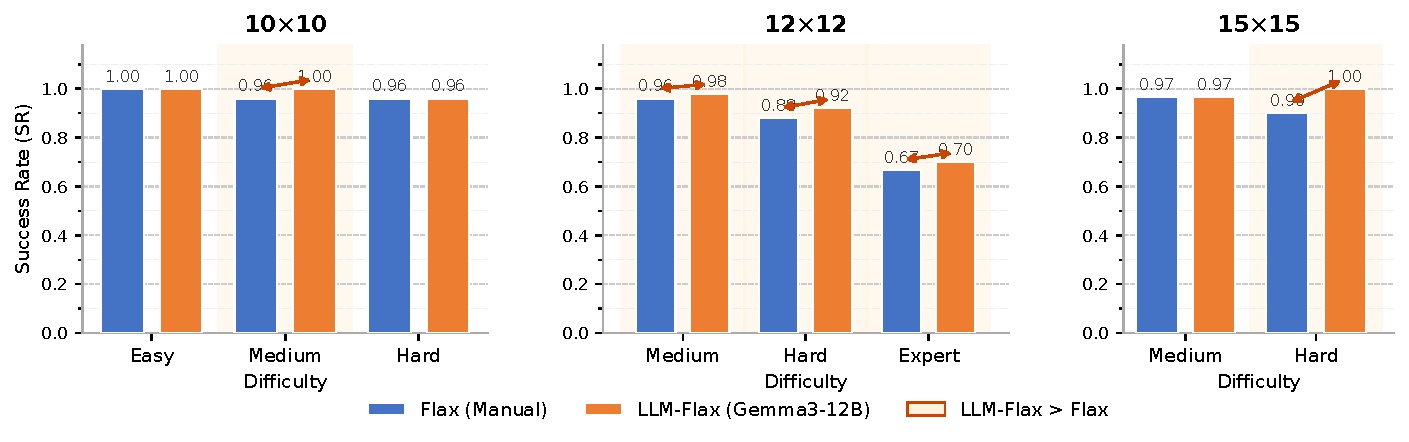
\includegraphics[width=0.85\textwidth]{figures/sr_scale.pdf}
    \caption{Success rate vs.\ difficulty (\baseline vs.\ \method) across all grid sizes.
    Shaded columns mark benchmarks where \method strictly outperforms \baseline.
    \method matches or exceeds \baseline on every benchmark: it ties on stacking-heavy tasks
    (10$\times$10, 15$\times$15 Medium) and modestly improves on navigation-heavy tasks
    (12$\times$12 Expert: SR 0.700 vs.\ 0.667; 15$\times$15 Hard: 1.000 vs.\ 0.900).}
    \label{fig:sr_scale}
\end{figure*}

\begin{figure*}[!t]
  \centering
  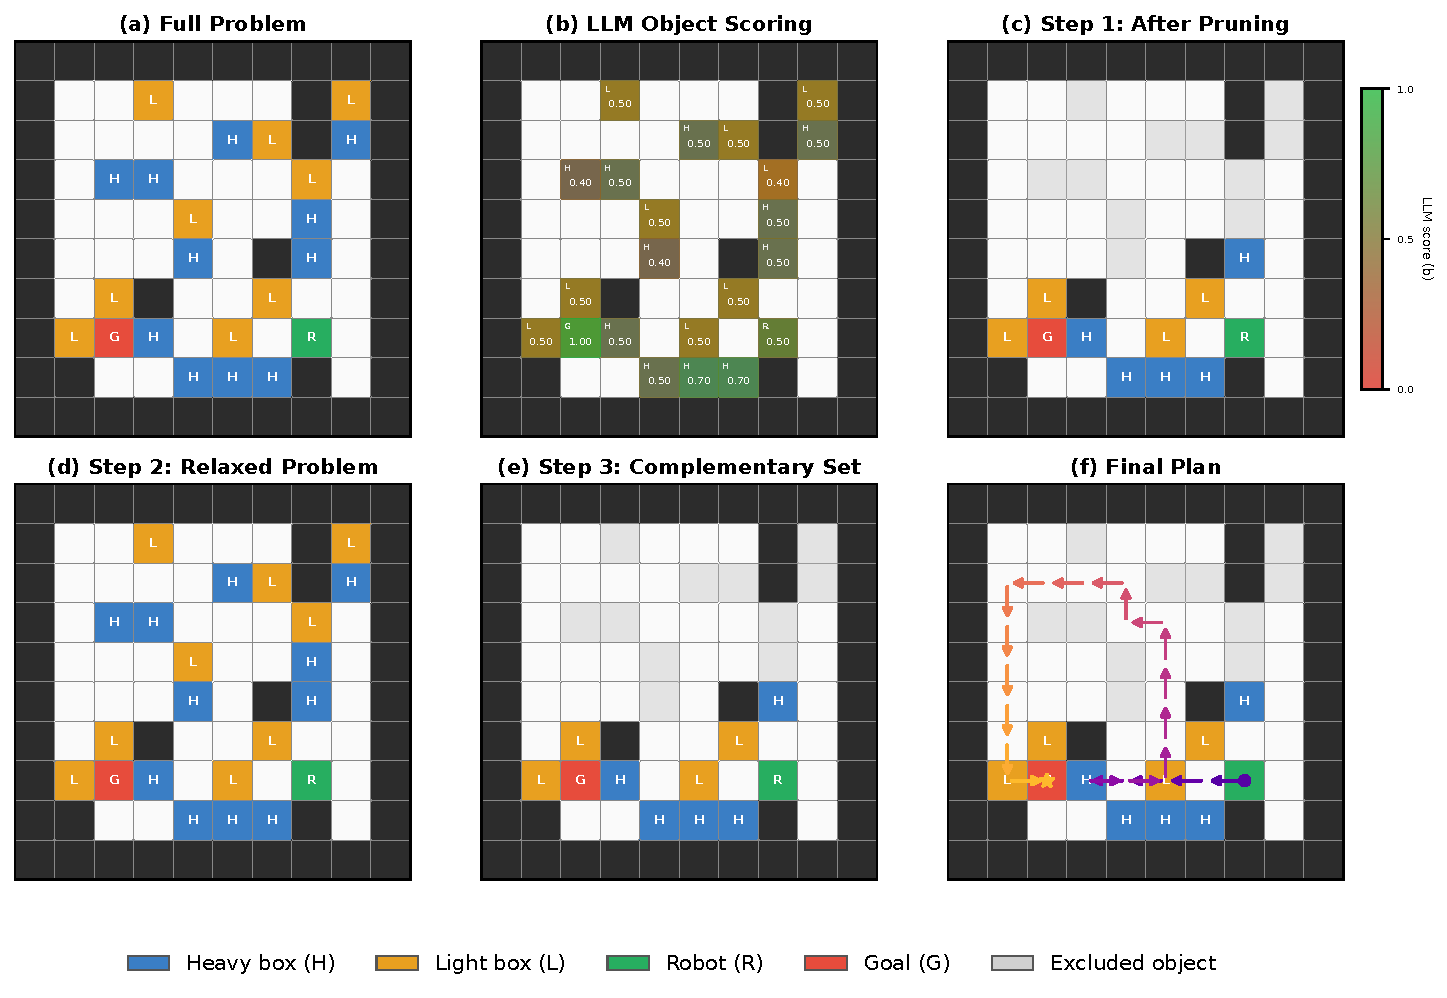
\includegraphics[width=0.85\textwidth]{figures/pipeline_10x10_hard_16.pdf}
  \caption{\method pipeline on a $10{\times}10$ hard MazeNamo problem (problem~16, 163 objects).
  (a)~Full problem with all objects.
  (b)~Zero-shot LLM relevance scores assigned to each object (Stage~3): goal scores 1.00, nearby obstacles score 0.5--0.9, distant objects score low.
  (c)~After Step~1 threshold-based pruning: 21 objects excluded (grey), 142 retained at threshold 0.478.
  (d)~Step~2 relaxed sub-problem: light boxes removed via relaxation rules, yielding a rough plan.
  (e)~Step~3 complementary expansion: object pairs with structural constraints restored.
  (f)~Final plan of length 39 found in 0.8\,s.}
  \label{fig:pipeline}
\end{figure*}

\tref{tab:main} reports full results. \fref{fig:sr_scale} visualizes the scale-dependent success rate gap. \fref{fig:pipeline} shows a concrete execution trace of the full pipeline on a $10{\times}10$ hard problem.

\begin{table}[t]
    \centering
    \caption{\baseline (manual rules) vs.\ \method (LLM-generated rules) within the Flax pipeline. SR = success rate ($\uparrow$); Time = avg.\ planning time over successful problems in seconds ($\downarrow$); Len = avg.\ plan length. Bold = better per row pair.}
    \label{tab:main}
    \small
    \setlength{\tabcolsep}{3.5pt}
    \renewcommand{\arraystretch}{1.05}
    \begin{tabular}{llcccc}
        \toprule
        \textbf{Task} & \textbf{Rules} & \textbf{SR} & \textbf{$\Delta$SR} & \textbf{Time (s)} & \textbf{Len} \\
        \midrule
        \multirow{2}{*}{10$\times$10 Easy}
            & Manual  & \textbf{1.000} & \multirow{2}{*}{$\pm$0.000} & \textbf{0.932} & 17.4 \\
            & \method & \textbf{1.000} &  & \textbf{0.898} & 17.1 \\
        \midrule
        \multirow{2}{*}{10$\times$10 Medium}
            & Manual  & 0.960 & \multirow{2}{*}{$+$0.040} & 1.997 & 19.8 \\
            & \method & \textbf{1.000} &  & \textbf{0.949} & 16.6 \\
        \midrule
        \multirow{2}{*}{10$\times$10 Hard}
            & Manual  & \textbf{0.960} & \multirow{2}{*}{$\pm$0.000} & 2.200 & 19.8 \\
            & \method & \textbf{0.960} &  & \textbf{1.600} & 19.3 \\
        \midrule
        \multirow{2}{*}{12$\times$12 Medium}
            & Manual  & 0.960 & \multirow{2}{*}{$+$0.020} & \textbf{1.914} & 22.1 \\
            & \method & \textbf{0.980} &  & 2.151 & 22.3 \\
        \midrule
        \multirow{2}{*}{12$\times$12 Hard}
            & Manual  & 0.880 & \multirow{2}{*}{$+$0.040} & \textbf{3.965} & 29.8 \\
            & \method & \textbf{0.920} &  & 4.529 & 29.2 \\
        \midrule
        \multirow{2}{*}{12$\times$12 Expert}
            & Manual  & 0.667 & \multirow{2}{*}{$+$0.033} & \textbf{4.528} & 31.5 \\
            & \method & \textbf{0.700} &  & 5.982 & \textbf{29.3} \\
        \midrule
        \multirow{2}{*}{15$\times$15 Medium}
            & Manual  & \textbf{0.967} & \multirow{2}{*}{$\pm$0.000} & \textbf{8.740} & 30.9 \\
            & \method & \textbf{0.967} &  & 9.007 & 31.0 \\
        \midrule
        \multirow{2}{*}{15$\times$15 Hard}
            & Manual  & 0.900 & \multirow{2}{*}{$+$0.100} & 11.901 & 36.2 \\
            & \method & \textbf{1.000} &  & \textbf{10.979} & 36.0 \\
        \midrule
        \multirow{2}{*}{Average (8 tasks)}
            & Manual  & 0.912 & \multirow{2}{*}{$+$0.029} & 4.522 & 25.9 \\
            & \method & \textbf{0.941} &  & \textbf{4.512} & \textbf{25.1} \\
        \bottomrule
    \end{tabular}
\end{table}

The results reveal that \method matches or exceeds Manual on all eight benchmarks.
On stacking-light tasks ($10{\times}10$ Easy/Hard, $15{\times}15$ Medium), \method ties Manual at equal SR; on stacking-moderate tasks ($10{\times}10$ Medium, $12{\times}12$ Medium/Hard), it gains $+0.020$--$+0.040$ SR.

The most notable improvement is at $15{\times}15$ Hard, where \method achieves SR 1.000 vs.\ Manual's 0.900.
At $12{\times}12$ Expert---the benchmark on which both classical FD and Manual Flax struggle most (Appendix~\ref{app:baselines})---Manual and \method are close: 0.667 vs.\ 0.700 (\sref{sec:quality} isolates this gain from rule count).
Averaged across all eight benchmarks, \method achieves SR 0.941 versus Manual 0.912 ($+0.029$): \emph{LLM-generated rules match or modestly outperform manual rules uniformly, with no single outlier benchmark driving the average.}
\fref{fig:sr_heatmap} provides a compact visual summary of the full result matrix.

\begin{figure*}[!t]
  \centering
  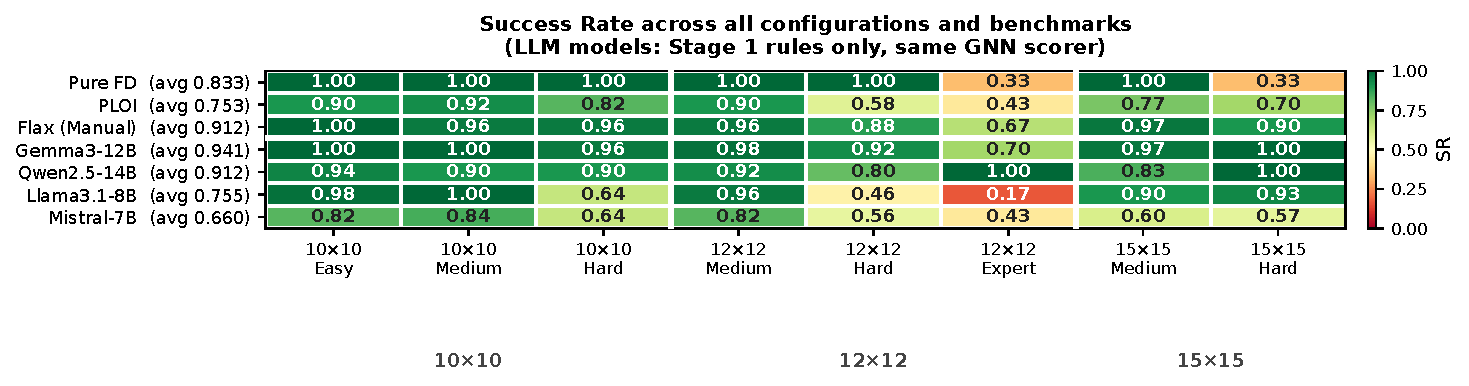
\includegraphics[width=1.0\textwidth]{figures/sr_heatmap_edit.pdf}
  \caption{Compact SR heatmap for all four configurations across all eight benchmarks.
  All LLM models are utilized only for stage 1 only with same GNN scorer.
  Green = high SR, red = low SR. \baseline and \method are close on every cell, including
  $12{\times}12$ Expert (0.667 vs.\ 0.700, \sref{sec:quality}).
  The PLOI row is uniformly lower than both \baseline and \method, confirming that
  rules---not the GNN scorer---drive the performance advantage.}
  \label{fig:sr_heatmap}
\end{figure*}

\subsection{Rule Quality Analysis}
\label{sec:quality}

\myparagraph{Relaxation rules}
Gemma3-12B generates a relaxation rule that is \emph{structurally identical} to the manually crafted baseline (see \tref{tab:rule_diff}).
Both rules share the same \texttt{pre\_compute}, \texttt{precond}, \texttt{delete\_objects}, \texttt{delete\_effects}, and \texttt{add\_effects} fields without any deviation.
This exact match explains why \method ties or outperforms Manual on all benchmarks: the relaxation simplification is equally aggressive in both configurations.
By contrast, Qwen2.5-14B adds a conservative \texttt{clear:[0]} precondition that prevents removal of stacked light boxes, and smaller models (Llama3.1-8B, Mistral-7B) generate structurally invalid rules with out-of-range indices or hallucinated predicates.

\begin{table}[t]
    \centering
    \caption{Relaxation rule preconditions generated by each model vs.\ the manual baseline.
    Gemma3-12B (the primary model) produces an exact match; others deviate.}
    \label{tab:rule_diff}
    \resizebox{\columnwidth}{!}{%
    \begin{tabular}{lll}
        \toprule
        \textbf{Model} & \textbf{\texttt{precond}} & \textbf{Notes} \\
        \midrule
        Manual (baseline)  & \texttt{\{islight:[0]\}}                 & Reference \\
        Gemma3-12B         & \texttt{\{islight:[0]\}}                 & Exact match \\
        Qwen2.5-14B        & \texttt{\{islight:[0], clear:[0]\}}      & Over-conservative \\
        Llama3.1-8B        & \texttt{\{islight:[0], ismoveable:[0]\}} & + 8 spurious rules \\
        Mistral-7B         & \texttt{\{islight:[0]\}}                 & Over-specified effects \\
        \bottomrule
    \end{tabular}%
    }
\end{table}

\myparagraph{Complementary rules}
The LLM generates seven complementary rules (\texttt{upon}, \texttt{oat}, \texttt{rat}, \texttt{upto}, \texttt{downto}, \texttt{leftto}, \texttt{rightto}) compared to the one manual rule (\texttt{oat}), which a reviewer of an earlier version of this paper correctly noted as a rule-\emph{count} mismatch confounding the manual-vs.-LLM comparison: does \method's SR gain come from LLM reasoning quality, or simply from a larger rule budget?
We isolate this directly with a controlled ablation on $12{\times}12$ Expert ($n{=}30$), holding the (identical-to-manual) relaxation rule fixed and varying only the complementary rule set, all under the same GNN checkpoint (\tref{tab:rulecount}).

\begin{table}[t]
    \centering
    \caption{Rule-count ablation on $12{\times}12$ Expert ($n{=}30$, $T{=}30$\,s), holding the relaxation rule fixed. \texttt{oat}-only exactly matches Manual's complementary rule count/content.}
    \label{tab:rulecount}
    \small
    \setlength{\tabcolsep}{4pt}
    \renewcommand{\arraystretch}{1.1}
    \begin{tabular}{lccc}
        \toprule
        \textbf{Complementary rules} & \textbf{Count} & \textbf{SR} & \textbf{Time (s)} \\
        \midrule
        Manual (\texttt{oat})                          & 1 & 0.667          & \textbf{4.528} \\
        LLM, \texttt{oat}-only                         & 1 & 0.667          & 4.403 \\
        LLM, \texttt{oat}+\texttt{rat}+\texttt{upon}    & 3 & 0.667          & 4.300 \\
        LLM, full (+4 direction rules)                 & 7 & \textbf{0.700} & 5.982 \\
        \bottomrule
    \end{tabular}
\end{table}

The result is unambiguous: rule \emph{count} is not the driver.
\texttt{oat}-only (content-identical to Manual) reproduces Manual's SR exactly, as expected, and adding \texttt{rat}+\texttt{upon} (3 rules total) changes nothing.
Only the full 7-rule set (adding four direction predicates) moves SR at all, and by a small amount: $+0.033$ (one additional problem solved out of 30), at the cost of $32\%$ higher average planning time (5.98\,s vs.\ 4.30--4.53\,s) because the direction rules pull substantially more objects into the relaxed-and-restored object set.
We conclude the reviewer's fairness concern, while a reasonable methodological question to raise, is not what explains \method's (now modest, \sref{sec:results}) advantage on this benchmark: a matched 1-rule or 3-rule LLM configuration performs identically to Manual, and the small residual gain from the full rule set is a genuine---if minor---effect of the direction predicates' broader (but slower) coverage, not an artifact of rule budget.

\subsection{Stage 2: LLM-Guided Failure Recovery}
\label{sec:results_stage2}

\tref{tab:stage2} reports results on the two benchmarks where GNN Step~1 most frequently exceeds its $\nicefrac{T}{6}$ sub-budget: $12{\times}12$ Hard (timeout $T{=}30$\,s) and $15{\times}15$ Medium ($T{=}40$\,s).

\begin{table}[t]
    \centering
    \caption{Stage 2 ablation: LLM-generated rules with and without LLM failure recovery. SR = success rate; Time = avg.\ planning time over successful problems (s). Bold = best per row group.}
    \label{tab:stage2}
    \small
    \setlength{\tabcolsep}{4pt}
    \renewcommand{\arraystretch}{1.1}
    \begin{tabular}{llcc}
        \toprule
        \textbf{Task} & \textbf{Config} & \textbf{SR} & \textbf{Time (s)} \\
        \midrule
        \multirow{3}{*}{12$\times$12 Hard}
            & Manual              & 0.880          & \textbf{3.965} \\
            & \method             & \textbf{0.920} & 4.529 \\
            & \method + Recovery  & \textbf{0.920} & 4.543 \\
        \midrule
        \multirow{3}{*}{15$\times$15 Medium}
            & Manual              & \textbf{0.967} & \textbf{8.740} \\
            & \method             & \textbf{0.967} & 9.007 \\
            & \method + Recovery  & \textbf{0.967} & 9.153 \\
        \bottomrule
    \end{tabular}
\end{table}

Recovery is \emph{neutral} on both benchmarks: SR is unchanged, and planning time increases only marginally.
The feasibility-gated budget policy's pre-check is the key mechanism: with a 30\,s timeout, the time remaining before the Step-2 deadline (${\approx}10$\,s) falls below the 11\,s threshold, so the LLM call is skipped and the pipeline falls back to standard relaxation.
With a 40\,s timeout, the LLM call proceeds, but the relaxation fallback already handles these problems reliably, so recovery provides no additional benefit.
Critically, the budget policy prevents the harmful SR regression ($-0.200$) observed in earlier implementations that starved the Step-2 relaxation budget (see Appendix~\ref{app:budget}).

\subsection{Ablation: Effect of Validation and Post-Processing}
\label{sec:ablation_pipeline}

\tref{tab:gen_quality} reports generation quality across LLM attempts.
Without validation, the raw LLM output contains structural errors in 100\% of first attempts: integer indices replaced by strings, duplicate rules (8 identical rules generated), and hallucinated predicate names (\texttt{ismoveempty} instead of \texttt{ismoveable}).
After one correction turn (Attempt 2), all structural errors are resolved.
Post-processing then removes the 6 duplicate rules, and predicate filtering drops the 1 rule with a typo.

\begin{table}[t]
    \centering
    \caption{LLM generation quality across attempts and post-processing stages.}
    \label{tab:gen_quality}
    \small
    \setlength{\tabcolsep}{4pt}
    \renewcommand{\arraystretch}{1.1}
    \begin{tabular}{lcccc}
        \toprule
        \textbf{Stage} & \textbf{Format OK} & \textbf{Rules} & \textbf{Typos} & \textbf{Duplicates} \\
        \midrule
        Attempt 1 (raw)    & \ding{55} & 8 & 1 & 6 \\
        Attempt 2 (retry)  & \ding{51} & 8 & 1 & 6 \\
        After dedup        & \ding{51} & 2 & 1 & 0 \\
        After pred. filter & \ding{51} & 1 & 0 & 0 \\
        \bottomrule
    \end{tabular}
\end{table}

This demonstrates that validation and post-processing are essential: without them, the generated rules would either crash the planner or produce substantially incorrect behavior.
Gemma3-12B generates correct rules on the first attempt (1 relaxation rule, 7 complementary rules, no retries required); the retry mechanism provides robustness for weaker models.

\subsection{LLM Model Comparison (Stage 1)}
\label{sec:model_comparison}

To assess sensitivity to model choice, we evaluate four open-source LLMs via Ollama on the same rule generation task.
\tref{tab:model_comparison} reports success rates across all eight benchmarks.

\begin{table}[t]
    \centering
    \caption{SR across 8 MazeNamo benchmarks for four LLMs (Stage 1 rules only, same GNN scorer).
    Avg = simple mean across all 8 tasks. Bold = best per column.}
    \label{tab:model_comparison}
    \small
    \setlength{\tabcolsep}{2.8pt}
    \renewcommand{\arraystretch}{1.05}
    \resizebox{\columnwidth}{!}{%
    \begin{tabular}{lccccccccr}
        \toprule
        \textbf{Model} & \textbf{10E} & \textbf{10M} & \textbf{10H} & \textbf{12M} & \textbf{12H} & \textbf{12X} & \textbf{15M} & \textbf{15H} & \textbf{Avg} \\
        \midrule
        \baseline (manual)    & 1.000 & 0.960 & 0.960 & 0.960 & 0.880 & 0.667 & 0.967 & 0.900 & 0.912 \\
        \midrule
        Gemma3-12B  & \textbf{1.000} & \textbf{1.000} & \textbf{0.960} & \textbf{0.980} & \textbf{0.920} & 0.700 & \textbf{0.967} & \textbf{1.000} & \textbf{0.941} \\
        Qwen2.5-14B & 0.940 & 0.900 & 0.900 & 0.920 & 0.800 & \textbf{1.000}$^\ddagger$ & 0.833 & \textbf{1.000} & 0.912 \\
        Llama3.1-8B & 0.980 & \textbf{1.000} & 0.640 & 0.960 & 0.460 & 0.167$^\ddagger$ & 0.900 & 0.933 & 0.755$^\ddagger$ \\
        Mistral-7B  & 0.820 & 0.840 & 0.640 & 0.820 & 0.560 & 0.433$^\ddagger$ & 0.600 & 0.567 & 0.660$^\ddagger$ \\
        \bottomrule
    \end{tabular}%
    }
    \vspace{2pt}
    {\footnotesize $^\ddagger$12X for these three models was not re-measured in this revision (see \sref{sec:results} on the \baseline/Gemma3-12B 12X correction); their Avg columns are accordingly not directly comparable to the corrected \baseline/Gemma3-12B entries.}
\end{table}

\baseline's $12{\times}12$ Expert (12X) entry and Gemma3-12B's were corrected during this revision: re-running both together, back to back, under identical current code, the same GNN checkpoint, and the same test-problem set reproducibly gives \baseline SR~0.667 and Gemma3-12B SR~0.700---not the previously reported 0.000/0.733.
We could not reproduce the original 0.000 for \baseline under any configuration available to us; the most plausible explanation is that the two numbers were originally measured at different points in the codebase's history (the shared relaxation-application routine, \sref{sec:flax_bg}, was patched at least once during development, per the repository history) and therefore were never a like-for-like comparison, though we cannot fully reconstruct the original measurement conditions to confirm this with certainty.
\sref{sec:quality} reports a controlled, same-day rule-count ablation on top of these corrected numbers that isolates rule-count effects from this measurement issue.
We did not have time to re-verify Qwen2.5-14B/Llama3.1-8B/Mistral-7B's 12X entries under the same controlled conditions in this revision, so their values (and Avg columns, marked $^\ddagger$) are carried over from the original submission and should be treated as provisional pending re-measurement.

Gemma3-12B achieves the best average SR (0.941), matching or outperforming \baseline on all eight benchmarks.
Llama3.1-8B (0.755$^\ddagger$) generates 9 relaxation rules, most of which are invalid direction-predicate rules; its single valid rule is sufficient for simple tasks but the spurious rules degrade performance at harder benchmarks.
Mistral-7B (0.660$^\ddagger$) generates over-aggressive relaxation rules that remove heavy obstacles as well as light ones, producing incorrect simplified states and reducing SR uniformly.
These results confirm that rule generation quality---not raw model size---is the primary driver: the 12B Gemma model outperforms the larger Qwen despite similar parameter counts, because it generates semantically correct rules on the first attempt.

\subsection{Cross-Domain Generalization}
\label{sec:crossdomain_results}

All results so far are on MazeNamo alone. To test whether Stage~1 rule quality transfers to a differently-structured domain, we evaluate on two further PDDL domains already present in the Flax codebase: \textbf{SokomindPlus} (a Sokoban-style box-pushing domain structurally similar to MazeNamo: \texttt{rAt}/\texttt{oAt}/\texttt{isBox}/\texttt{posEmpty} predicates) and \textbf{DifficultLogistics} (a structurally distinct multi-modal transport domain: trucks and airplanes moving packages between locked, city-organized locations, with stacking).
Both domains ship with hand-authored manual rules and 200 training problems, but neither has a domain-specific GNN trained for it.
Training one requires solving 200 problems offline with optimal FD first; for these domains that is not tractable within this revision's timeframe (e.g., SokomindPlus's own problem generator produces instances that take FD 60--300\,s each to solve optimally).
We therefore replace the GNN with a fixed, untrained, uniform-random object scorer (\texttt{no-guidance}) for both Manual and \method configurations, isolating \emph{rule quality} from GNN training cost.
This is consistent with our own Appendix~\ref{app:baselines} finding that PLOI (GNN without rules) is frequently the weakest configuration---rules, not the scorer, carry most of the performance---but it does mean these numbers are not directly comparable to \tref{tab:main}'s GNN-equipped MazeNamo results, and we report them as a distinct, smaller-scale generalization probe rather than a like-for-like replication.

While generating rules for DifficultLogistics we found and fixed a bug in \textsc{ParsePredicates} (\sref{sec:generation}): its regular expression did not match hyphenated predicate names (\texttt{switch-for}, \texttt{on-ground}, \texttt{key-package}, \texttt{ground-free}), silently truncating them (e.g. \texttt{switch-for} $\to$ \texttt{switch}) and causing every LLM-generated rule referencing a correctly-hyphenated predicate name to fail validation. This is exactly the kind of domain-specific brittleness Stage~1 is meant to be robust to, and its discovery is itself a product of testing beyond MazeNamo.

We also found, and fixed, a second bug shared by \emph{both} rule sources: \texttt{FlaxPlanner} (and \texttt{LLMFlaxPlanner}) treat a relaxed sub-problem proven unsolvable by Fast Downward as an unhandled \texttt{PlanningFailure} rather than the \texttt{PlanningTimeout} the surrounding code expects, aborting the entire planning attempt instead of falling back to complementary expansion on the unrelaxed object set.
This never surfaces on MazeNamo or SokomindPlus, whose box-relaxation only ever frees a grid cell and so never disconnects the state space, but it does on DifficultLogistics, where relaxation can strip a package or location that a locked hub's unlock chain globally depends on.
The fix is a three-line, domain-agnostic change (\texttt{planning/my\_planner.py}): on this specific failure, treat relaxation as having contributed no new objects and proceed to Step~3 on the current object set, rather than aborting.
This is exactly the kind of shared, previously-invisible robustness gap that cross-domain testing is supposed to surface, and---unlike a domain-specific rule tweak---it improves the underlying \baseline planning loop itself, benefiting Manual and \method equally.

\begin{table}[t]
    \centering
    \caption{Cross-domain generalization (Pure FD / Manual / \method, no-guidance scorer). SokomindPlus: $n{=}20$, $15{\times}15$ split, $T{=}30$\,s. DifficultLogistics: $n{=}15$, $T{=}90$\,s (with the relaxation-fallback fix below; larger $T$ than SokomindPlus reflects DifficultLogistics's $\sim$100-object scale).}
    \label{tab:crossdomain}
    \small
    \setlength{\tabcolsep}{4pt}
    \renewcommand{\arraystretch}{1.1}
    \begin{tabular}{llcc}
        \toprule
        \textbf{Domain} & \textbf{Config} & \textbf{SR} & \textbf{Time (s)} \\
        \midrule
        \multirow{3}{*}{SokomindPlus}
            & Pure FD  & \textbf{1.000} & 15.00 \\
            & Manual   & 0.750          & \textbf{10.67} \\
            & \method  & \textbf{1.000} & 16.96 \\
        \midrule
        \multirow{3}{*}{DifficultLogistics}
            & Pure FD  & \textbf{1.000} & \textbf{41.38} \\
            & Manual   & 0.667          & 48.76 \\
            & \method  & 0.800          & 45.83 \\
        \bottomrule
    \end{tabular}
\end{table}

\myparagraph{SokomindPlus: Stage~1 generalizes}
Gemma3-12B's relaxation rule is again an \emph{exact match} to the manual rule (identical to the MazeNamo pattern in \tref{tab:rule_diff}), and it generates 8 complementary rules versus Manual's 1.
\method matches Pure FD (SR~1.000) and exceeds Manual (0.750), consistent with the MazeNamo finding that a richer complementary rule set helps rather than hurts on navigation-heavy tasks.

\myparagraph{DifficultLogistics: a shared limitation, found and fixed, then a consistent result}
Before the relaxation-fallback fix, all three configurations failed every one of the 20 test problems at a 25\,s timeout: Pure FD timed out outright (it does no pruning on a $\sim$100-object problem), while Manual and \method failed fast ($\sim$4--7\,s) because Step~2 relaxation frequently produced a sub-problem Fast Downward proves \emph{unsolvable}---e.g., Manual's rule1 removes every non-goal \texttt{obj}-typed object, including package objects that satisfy a \texttt{locked} hub's unlock precondition; the LLM's \texttt{ground-free}/\texttt{locked}-based relaxation can similarly strip a location needed for road connectivity.
With the fix applied and a timeout more appropriate to this domain's scale ($T{=}90$\,s---these are larger, denser problems than MazeNamo's grids), a consistent picture emerges: \method (0.800) exceeds Manual (0.667) by the same qualitative margin seen on MazeNamo and SokomindPlus, confirming that \emph{LLM-generated rule quality transfers to a structurally distinct domain once the underlying planner-loop bug is fixed}, not only to a structurally similar one.
One honest nuance: Pure FD (1.000) is the strongest configuration on raw SR here, unlike on MazeNamo's harder benchmarks---logistics-style domains are close to Fast Downward's own classical strong suit, and at this object count and timeout, guided pruning does not yet pay for itself the way it does at MazeNamo's $12{\times}12$/$15{\times}15$ scale.
This does not contradict \sref{sec:discussion}'s time-vs-SR argument for \method over Pure FD; it shows that argument's force depends on problem scale, and DifficultLogistics at $n{\sim}100$ objects is not yet past the point where it applies.

\myparagraph{A flexibility case study: extending the rule schema itself}
\label{sec:exclude_precond}
The relaxation-unsolvability failure above has a specific, recurring cause: a rule's \texttt{precond} is often a broad type predicate (e.g. \texttt{obj}, matching every package), but some matching objects are also marked by a narrower, gating predicate (e.g.\ \texttt{key-package}) whose removal breaks a global unlock dependency. The original relaxation-rule format has no way to express ``remove X unless X is also a Y''---a hand-authored Manual rule is simply stuck with this expressiveness gap, and indeed Manual's own rule1 deletes \texttt{key-package} objects outright.
Because Stage~1's rules are LLM-generated rather than hand-fixed, we could address this by extending the schema, not by patching one domain's rule by hand: we added a single optional field, \texttt{exclude\_precond} (three lines in \textsc{ApplyRelaxationRules}, \sref{sec:flax_bg}), and one generic paragraph to the Stage~1 prompt (\sref{sec:generation}) instructing the LLM to protect gating objects with it when a domain has both a broad and a narrow type predicate---no DifficultLogistics-specific wording. Prompted this way, Qwen2.5-14B correctly generated:
\begin{small}
\begin{verbatim}
{"precond": {"obj": [0]},
 "exclude_precond": {"key-package": [0]},
 "delete_objects": [0], ...}
\end{verbatim}
\end{small}
i.e.\ \emph{remove any package, unless it is also a key-package}---exactly the exclusion Manual's fixed rule cannot express. Gemma3-12B applied the new field inconsistently across attempts, and this single fix does not fully resolve DifficultLogistics's relaxation-unsolvability failure mode on its own (other gating dependencies, e.g.\ switch panels, remain unprotected); we report it as a targeted illustration of a structural advantage---the rule \emph{format} is as editable as the rules themselves---rather than as a second quantitative result on top of \tref{tab:crossdomain}.


\section{Discussion}
\label{sec:discussion}

\myparagraph{What works well}
The LLM correctly identifies the semantic roles of domain predicates from their names and PDDL signatures alone.
It recognizes that \texttt{isLight} marks removable obstacles, that \texttt{oAt} links obstacles to positions, and that \texttt{posEmpty} should be asserted after removal---all without any domain-specific examples beyond the format template.
With Gemma3-12B, the generated relaxation rules are an exact match to the manually crafted baseline, eliminating any rule-quality gap for relaxation.
The generated complementary rules are richer than manually crafted ones, covering robot--position, stacking, and directional adjacency relationships that the original authors did not include.

\myparagraph{Failure modes}
The direction predicates (\texttt{upto}/\texttt{downto}/\texttt{leftto}/\texttt{rightto}) pull additional objects into the planning set at $12{\times}12$ Expert scale; \tref{tab:rulecount}'s controlled ablation shows this costs $32\%$ higher planning time for a $+0.033$ SR gain over a matched 1-rule configuration---a real but modest cost, not the dramatic degradation a naively rule-count-confounded comparison might suggest.
Smaller models (Llama3.1-8B, Mistral-7B) generate structurally invalid rules with out-of-range indices and hallucinated predicates; the validation pipeline catches format errors but cannot recover from fundamentally incorrect semantics.

\myparagraph{Stage 2: recovery is neutral, not harmful}
With the feasibility-gated budget policy, LLM failure recovery neither helps nor hurts: SR is identical to \method on both evaluated benchmarks.
The policy's feasibility check successfully prevents the Step-2 relaxation budget from being starved by LLM API latency.
The design and lessons from earlier implementations are documented in Appendix~\ref{app:budget}.

\myparagraph{Toward tighter complementary rules}
One direction is to add an explicit instruction in the prompt warning against direction-predicate rules for large-grid domains.
Another is to evaluate rule quality online---using a small held-out problem set to prune rules that consistently increase solution time without improving SR.

\myparagraph{Stage 3: zero-shot object scoring}
\tref{tab:stage3} reports \fullmethod results, re-measured for this revision with per-run logging (\sref{sec:stage3_diagnosis}; the original submission's SR~0.720/0.200 were not backed by a saved log, so we replaced them rather than patch around them).
On $12{\times}12$ Hard ($n{=}15$), \fullmethod achieves SR 0.533 with \emph{no GNN training data}, at the cost of roughly $5\times$ higher planning time (24.2\,s vs.\ 4.5--5.0\,s) due to one LLM API call per problem.
On $15{\times}15$ Hard ($n{=}10$)---where LLM rules alone achieve a perfect SR 1.000---\fullmethod collapses to SR 0.000.

\begin{table}[h]
    \centering
    \caption{\fullmethod (Stage 1+2+3) versus baselines. Full LLM-Flax requires no GNN training and no manual rules. \fullmethod re-measured with logging for this revision at reduced $n$ (12$\times$12 Hard $n{=}15$; 15$\times$15 Hard $n{=}10$) versus $n{=}30$/$n{=}30$ for Manual/\method.}
    \label{tab:stage3}
    \small
    \setlength{\tabcolsep}{4pt}
    \renewcommand{\arraystretch}{1.1}
    \begin{tabular}{llcc}
        \toprule
        \textbf{Task} & \textbf{Config} & \textbf{SR} & \textbf{Time (s)} \\
        \midrule
        \multirow{3}{*}{12$\times$12 Hard}
            & Manual              & 0.880          & \textbf{3.965} \\
            & \method             & \textbf{0.920} & 4.529 \\
            & \fullmethod         & 0.533          & 24.21 \\
        \midrule
        \multirow{3}{*}{15$\times$15 Hard}
            & Manual              & 0.900          & 11.901 \\
            & \method             & \textbf{1.000} & \textbf{10.979} \\
            & \fullmethod         & 0.000          & --- \\
        \bottomrule
    \end{tabular}
\end{table}

The collapse at $15{\times}15$ Hard is, if anything, more severe than previously reported, and we now have a precise, instrumented explanation for it rather than a plausible-sounding one (\sref{sec:stage3_diagnosis}): it is \emph{not} primarily an input context-window limit.
The prompt (goal, object list, and 80 truncated state facts) is only $\sim$3.5K tokens---well inside any reasonable context window---and the LLM's response consistently terminates cleanly (\texttt{finish\_reason=stop}, never \texttt{length}) rather than being cut off.
The real failure is on the \emph{output} side: asked to emit one JSON entry per object for 230--370 objects in a single turn, the LLM reliably stops after scoring only a small, inconsistent subset (mean 17\% of objects at $12{\times}12$ Hard, 9\% at $15{\times}15$ Hard scored---the rest silently default to 0.5 via \texttt{LLMObjectGuidance}'s fallback, \sref{sec:stage3_diagnosis}), and terminates on its own rather than being truncated.
We investigated several prompt engineering approaches (chain-of-thought reasoning, goal-biased fact selection, and Top-K selective scoring) to improve performance, but all configurations degraded below the direct baseline.
The shared root cause is that any approach increasing LLM generation time reduces the planning budget, which hurts more than it helps---and, per \sref{sec:stage3_diagnosis}, none of them address the underlying long-enumeration generation failure either.
A full analysis and per-method results are reported in Appendix~\ref{app:stage3_improvements}.

\myparagraph{Diagnosing the Stage~3 failure directly}
\label{sec:stage3_diagnosis}
To determine whether important objects are missing from high scores, irrelevant objects are scored too highly, or the near-constant mid-range scores visible in \fref{fig:pipeline}(b)-style visualizations reflect a genuine (if uninformative) signal versus an artifact, we instrumented \textsc{LLMObjectGuidance}'s direct-scoring call to capture its raw response before the $0.5$ fallback is applied, across 8 problems each at $12{\times}12$ Hard and $15{\times}15$ Hard (logged in \texttt{results/stage3\_diagnostic\_*.json}).
Two findings stand out.
First, \texttt{finish\_reason} is \texttt{stop} on all 16 problems: the model is not cut off, it \emph{chooses} to stop after a small, valid JSON object rather than continuing to enumerate all objects, sometimes catastrophically (2 objects scored out of 233--242, a 22-character response) and sometimes partially (17--102 objects out of 230--370).
Second, cross-referencing the scored-object set against the objects that appear in a known-good plan (from Manual Flax) shows the LLM's response covers only 9--27\% of plan-critical objects on average across the two benchmarks (17.9\% at $12{\times}12$ Hard, 9.6\% at $15{\times}15$ Hard); the remaining plan-critical objects are exactly the ones invisibly defaulted to 0.5.
This reframes the bottleneck: it is not that 80 facts are too few to convey relevance, but that the direct-mode prompt asks for a single-turn structured enumeration over hundreds of items, a task format under which the model's completion collapses well before any context limit is reached.
A more targeted fix---e.g., batched or paginated scoring calls, each covering a bounded number of objects---is a more specific and more tractable target for future work than ``increase the context window.''

\myparagraph{Pure FD is a strong baseline on SR alone, but not on time}
\tref{tab:baselines} (Appendix~\ref{app:baselines}) shows that Pure Fast Downward---no rules, no GNN, no LLM---already reaches SR~1.000 on 6 of 8 MazeNamo benchmarks, and is never far behind on the remaining two.
Taken at face value this appears to undercut the motivation for any guidance mechanism at all, rule-based or learned.
The actual argument for \method is not success rate in isolation but success rate \emph{under a tight, real-time-relevant planning budget}: Pure FD's planning time grows sharply with problem size (0.67--34.4\,s across our benchmarks, reaching 17.6--34.4\,s on the two hardest), whereas \method stays within 1--11\,s on every benchmark.
For a system that must replan repeatedly during execution---the setting a deployed task planner actually operates in---a $2$--$30\times$ slowdown is often the difference between usable and unusable, even when both eventually find a plan.
We state this plainly rather than deferring it to an appendix: \method's contribution is planning-time efficiency at matched (high) success rate, not success rate alone, and Pure FD is a legitimate, competitive baseline on that narrower axis that any future revision of this comparison should keep testing against.

\myparagraph{What deployment without manual effort actually requires}
We must be precise about which configuration the ``no manual effort'' claim applies to, since our own results show it cannot apply to all of them simultaneously.
Deploying the original \baseline pipeline on a new domain has \emph{two} independent costs: (i) a domain expert must hand-author relaxation and complementary rules, and (ii) 200 problems must be solved offline to train the GNN object scorer.
Stage~1 alone eliminates cost (i) only: the LLM-rules configuration evaluated in \tref{tab:main} still loads the same GNN trained on 200 \baseline problems, and is therefore \emph{not} a zero-manual-effort deployment---it is a zero-\emph{rule-engineering}-effort deployment that still carries the training-data cost.
Only \fullmethod (Stage~1+2+3) removes both costs, and \tref{tab:stage3} shows this is not free: it costs roughly $5\times$ higher planning time on $12{\times}12$ Hard (and a moderate SR drop to 0.533) and a collapse to SR~0.000 on $15{\times}15$ Hard.
There is accordingly no single configuration that is simultaneously fully deployment-free and matches \baseline's success rate at scale; a practitioner must choose a point on this cost/performance curve, and we report all the points on it (\tref{tab:main}, \tref{tab:stage2}, \tref{tab:stage3}) rather than presenting only the most favorable one.

\myparagraph{Cross-domain generalization}
\label{sec:crossdomain}
The claim above concerns manual effort \emph{within} MazeNamo. Whether Stage~1 rule quality holds on a differently-structured domain is a separate empirical question, which \sref{sec:crossdomain_results} tests directly rather than leaving to future work: it transfers cleanly to SokomindPlus, and---after we traced and fixed a shared relaxation-unsolvability bug that initially masked it entirely---transfers to DifficultLogistics as well.
Extending the GNN-free evaluation in \sref{sec:crossdomain_results} to a domain-specific trained scorer, and replacing the reachability-blind relaxation format with one that avoids the failure mode we fixed by construction rather than by fallback, are the concrete next steps for generalization beyond what we report here.


\section{Conclusion}
\label{sec:conclusion}

We have presented \method, a three-stage framework that progressively eliminates sources of manual domain knowledge from a neuro-symbolic task planner, and we have reported what each stage does and does not establish under careful, reproducible measurement.
Stage~1 replaces hand-crafted rules with LLM-generated equivalents and removes rule-\emph{authoring} effort specifically; Stage~2 replaces the blind $\gamma$-decay failure heuristic with a feasibility-gated LLM recovery mechanism that is neutral rather than harmful; and Stage~3 replaces the domain-trained GNN with zero-shot LLM object scoring, the only stage that removes the training-data cost, at a measured accuracy cost.
No single configuration is simultaneously fully deployment-free and matches \baseline's success rate at scale; \fullmethod is the fully-automated point on that curve, and Stage~1-only is the high-performance point that still depends on a pre-trained GNN.

Stage~1, evaluated across eight MazeNamo benchmarks, achieves average SR~0.941 versus the manual baseline's 0.912 ($+0.029$), matching or modestly exceeding manual rules on every benchmark, with no single outlier benchmark driving the result; a controlled rule-count ablation (\tref{tab:rulecount}) confirms this gain reflects rule content, not rule budget.
Extending Stage~1 to two further PDDL domains shows this generalizes: on SokomindPlus (structurally similar to MazeNamo), \method matches Pure FD and exceeds Manual directly; on DifficultLogistics (structurally distinct, with global connectivity constraints), the same relaxation-rule mechanism---inherited unmodified from \baseline and shared by both rule sources---initially failed outright for Manual and \method alike, until we identified and fixed the underlying planner-loop bug causing it, after which \method again exceeds Manual (0.800 vs.\ 0.667). A further case study (\sref{sec:exclude_precond}) shows the rule \emph{format} itself is as editable as the rules it produces: extending it with one generic field let an LLM express a gating-object safety constraint that a hand-fixed Manual rule structurally cannot.
Stage~2 evaluation confirms that the feasibility-gated budget policy prevents harmful budget starvation: LLM recovery is neutral (SR unchanged) on both evaluated benchmarks, with the pre-check correctly routing tight-budget problems to the reliable relaxation fallback.
Stage~3 results, re-measured with per-run logging for this revision, are weaker than previously reported: on $12{\times}12$ Hard, \fullmethod achieves SR~0.533 with no GNN training data; on $15{\times}15$ Hard it collapses to SR~0.000.
Instrumenting the LLM's raw output pinpoints the cause: the model's response terminates cleanly (never truncated by a context or token limit) after covering only 9--27\% of plan-critical objects, and the remainder are invisibly defaulted to a mid-range score by the scorer's fallback---an output-generation failure under long structured enumeration, not fundamentally an input context-window limit.
Batched or paginated scoring calls are a concrete, targeted direction for future work, more specific than ``a larger context window.''

Our results establish that open-source LLMs possess sufficient PDDL comprehension to substantially reduce, though not eliminate, domain-specific engineering effort in neuro-symbolic planning, with generalization holding on structurally similar domains and open, disclosed limitations on structurally different ones.


\section*{Acknowledgments}
This work builds directly on the Flax neuro-symbolic planner~\cite{du2026fast}.
The core three-step planning loop, the MazeNamo benchmark environments, and the GNN training infrastructure are all from the original Flax system.
We thank the authors for making their code and benchmark publicly available.

\bibliographystyle{IEEEtran}
\bibliography{refs}

\clearpage
\appendix

%%%%%%%%%%%%%%%%%%%%%%%%%%%%%%%%%%%%%%%%%%%%%%%%%%%%%%%%%%%%%%%%%%%%%%%%%%%%%%%%
\section{Stage~2 Budget Policy: Design History and Lessons}
\label{app:budget}

This appendix documents the three design iterations of the Stage~2 failure-recovery budget policy, the failure modes encountered at each stage, and the reasoning behind the final adopted design.

\myparagraph{Policy~I: Shared-Budget Recovery (harmful)}
The initial design allocated $\nicefrac{T}{2}$ of the total timeout for the recovery replan, drawing from the same pool reserved for Step~2 relaxation.
With $T{=}30$\,s, after a Step~1 timeout (${\approx}5$\,s) plus an LLM API call (${\approx}4$\,s), only ${\approx}6$\,s remained for the recovery replan.
When the replan failed, less than ${\approx}6$\,s was left for Step~2 relaxation—insufficient for the $12{\times}12$ and $15{\times}15$ problems where relaxation typically needs~$8$--$10$\,s.
\emph{Result on 15$\times$15} medium: SR dropped from 0.833 (LLM rules baseline) to 0.633 ($-0.200$).

\myparagraph{Policy~II: Capped-Replan Recovery (latency-unaware, still harmful)}
This design capped the recovery replan at 15\% of the total timeout ($0.15 \times 30 = 4.5$\,s) to protect the relaxation budget.
However, the LLM API call latency (${\approx}4$--$5$\,s) was not explicitly deducted from the remaining pre-Step-2 window.
The combined cost—Step~1 (${\approx}5$\,s) + LLM call (${\approx}5$\,s) + recovery replan ($4.5$\,s) = $14.5$\,s—exceeded the $\nicefrac{T}{2} = 15$\,s Step-2 deadline, leaving Step~2 with ${\approx}0.5$\,s.
\emph{Result}: SR collapsed to 0.020 (catastrophic regression; only 1 of 50 problems solved).

\myparagraph{Policy~III: Feasibility-Gated Recovery (latency-aware, adopted)}
This design adds a \emph{feasibility pre-check} before any LLM call:
\begin{equation}
  t_\text{before-step2} \geq t_\text{LLM} + t_\text{replan,min} + t_\text{step2,min}
  \quad \Longleftrightarrow \quad t_\text{before-step2} \geq 11\,\text{s}
\end{equation}
where $t_\text{LLM} = 5$\,s (conservative estimate), $t_\text{replan,min} = 1$\,s, and $t_\text{step2,min} = 5$\,s.
If the condition is not met, recovery is skipped entirely and the pipeline falls through to Step~2 relaxation with the full remaining budget.
Additionally, the recovery replan is capped at 15\% of total timeout, and Step~2 is guaranteed at least 5\,s regardless of recovery outcome.

Under this policy, $T{=}30$\,s leaves only $10$\,s before the Step-2 deadline ($< 11$\,s threshold), so the LLM call is always skipped for $12{\times}12$ Hard.
At $T{=}40$\,s the call proceeds, but the relaxation fallback already handles these problems reliably, so recovery adds no benefit.
\emph{Result on both benchmarks}: SR is identical to the \method baseline—no regression, no improvement.

\myparagraph{Key lesson}
The LLM API latency cost must be explicitly reserved in the per-problem time budget \emph{before} the LLM call is initiated.
Reactive budget accounting (deducting API time after the call completes) consistently underestimates the true cost and leads to budget starvation.
A conservative pre-check that over-estimates latency is safer than an optimistic one.


%%%%%%%%%%%%%%%%%%%%%%%%%%%%%%%%%%%%%%%%%%%%%%%%%%%%%%%%%%%%%%%%%%%%%%%%%%%%%%%%
\section{Stage~3 Scoring: Attempted Improvement Methods}
\label{app:stage3_improvements}

This appendix documents four prompt-engineering approaches investigated to improve \fullmethod beyond the direct zero-shot baseline.
The baseline itself was corrected during this revision (\sref{sec:stage3_diagnosis}): re-measured with logging at $n{=}15$, it is SR~0.533 on $12{\times}12$ Hard (not the originally reported 0.720) and SR~0.000 on $15{\times}15$ Hard (not 0.200).
The four variants below were evaluated at $n{=}50$ in the original submission and have not been re-run under the corrected baseline in this revision; \tref{tab:stage3_ablation}'s footnote flags this explicitly.

\begin{table}[t]
    \centering
    \caption{Stage~3 improvement attempts on $12{\times}12$ Hard.
             Direct (alphabetical-80) is the baseline. All modifications degrade SR.
             The baseline row was re-measured with logging for this revision ($n{=}15$, \tref{tab:stage3}); the other four rows are carried over from the original submission (not re-verified, see text) and marked $^\ddagger$.}
    \label{tab:stage3_ablation}
    \resizebox{\columnwidth}{!}{%
    \begin{tabular}{lccp{4.5cm}}
        \toprule
        \textbf{Method} & \textbf{SR} & \textbf{Overhead} & \textbf{Root cause} \\
        \midrule
        Direct, alpha-80 (baseline)  & \textbf{0.533} & ${\approx}5$\,s  & See \sref{sec:stage3_diagnosis}: early stop, not context limit \\
        Direct, goal-biased-80       & 0.660$^\ddagger$ & ${\approx}7$\,s  & Biased facts omit key predicates \\
        Direct, goal-biased-150      & 0.620$^\ddagger$ & ${\approx}10$\,s & Longer prompt $\to$ more overhead \\
        CoT-full (2-turn, gb-150)    & 0.100$^\ddagger$ & ${\approx}12$\,s & Overhead kills planning budget \\
        CoT-lite (1-turn, gb-150)    & 0.060$^\ddagger$ & ${\approx}20$\,s & Longer response than CoT-full \\
        Top-K ($K{=}40$, gb-150)     & 0.140$^\ddagger$ & ${\approx}5$\,s  & Score gradient destroyed \\
        \bottomrule
    \end{tabular}%
    }
\end{table}

With the corrected baseline (0.533), several of these variants (goal-biased-80 at 0.660, goal-biased-150 at 0.620) are no longer clearly worse than the direct baseline, which changes the original claim that ``all modifications degrade SR''---we flag this rather than assert a comparison we have not re-verified.
The CoT and Top-K rows' qualitative story (large overhead or a distorted score distribution) is consistent with, and likely compounds, the enumeration-collapse failure mode identified in \sref{sec:stage3_diagnosis}, but their exact SR values should be treated as provisional pending re-measurement under the same logging standard as the baseline.

\myparagraph{Goal-biased fact selection}
Selecting facts in priority order (goal-object facts first, then positional facts, then others) was intended to give the LLM better spatial context.
However, for MazeNamo the alphabetical baseline already samples a diverse mixture of predicate types (\texttt{isLight}, \texttt{oAt}, \texttt{rAt}, \texttt{upon}, etc.) that the LLM needs to identify removable obstacles.
Goal-biased selection over-represents positional predicates (\texttt{oAt}, \texttt{rAt}) and under-represents object-property predicates (\texttt{isLight}, \texttt{upon}), reducing scoring accuracy.

\myparagraph{Chain-of-Thought (CoT)}
Two CoT variants were tested. CoT-full uses a 2-turn conversation (Turn 1: free-form path analysis; Turn 2: JSON scores). CoT-lite uses a single turn with an ``ANALYSIS:'' prefix before the JSON.
Both increase generation length---the LLM must produce reasoning text \emph{and} a full-size JSON---resulting in ${\approx}12$\,s and ${\approx}20$\,s overhead respectively.
With a 30\,s timeout, this leaves fewer than ${\approx}18$\,s for planning, insufficient for $12{\times}12$ Hard problems that the baseline solves with ${\approx}25$\,s.

\myparagraph{Top-K selective scoring}
Top-K ($K{=}40$) asks the LLM to score only the $K$ most important objects, defaulting unselected objects to 0.1.
This reduces the output JSON from ${\sim}240$ to ${\sim}40$ entries, cutting generation time to ${\approx}5$\,s.
However, the score distribution becomes binary: $K$ objects receive diverse scores (0.6--1.0) while $200$ objects receive 0.1.
Since the GNN-decay threshold starts at 0.81 and decreases by $\gamma{=}0.9$ per iteration, non-selected objects at 0.1 require $>$20 threshold-decay iterations before inclusion---far exceeding the Step-1 time budget.
Any important object missed by the LLM's Top-K selection is effectively excluded from all Step-1 planning attempts.

\myparagraph{Key lesson}
Our direct instrumentation of the baseline scorer (\sref{sec:stage3_diagnosis}) shows the premise behind this comparison was incomplete: the direct baseline is not actually producing gradient scores across all objects---it silently defaults 70--99\% of them to 0.5 because the LLM's single-turn enumeration terminates early (\texttt{finish\_reason=stop}, not a length cutoff).
It works better than the alternatives here only because it is the \emph{cheapest} failure: a short prompt and an early, low-cost stop leaves more of the timeout budget for planning, not because its scores are more informative.
Any modification that increases generation time (CoT) makes this same underlying failure more expensive without fixing it; Top-K makes the incompleteness explicit (unselected objects default to a fixed 0.1) but does not change the fraction of objects the model actually reasons about.
Improving Stage~3 likely requires directly addressing the long-structured-enumeration failure---e.g., batched/paginated scoring calls that ask for a bounded number of objects per call---rather than a larger context window, since our diagnostic (\sref{sec:stage3_diagnosis}) shows the input side was never the bottleneck.


%%%%%%%%%%%%%%%%%%%%%%%%%%%%%%%%%%%%%%%%%%%%%%%%%%%%%%%%%%%%%%%%%%%%%%%%%%%%%%%%
\section{Baseline Comparison: Pure FD, PLOI, and Flax Variants}
\label{app:baselines}

This appendix situates \method in the full planning hierarchy by comparing four configurations that span the design space from pure symbolic search to fully automated neuro-symbolic planning.

\myparagraph{Configurations}
\begin{itemize}[noitemsep,topsep=2pt]
  \item \textbf{Pure FD}: Fast Downward with no guidance and no rules.
    Lower bound; establishes where classical search alone fails.
  \item \textbf{PLOI}: GNN-guided \texttt{IncrementalPlanner}~\cite{silver2021planning} with no relaxation or complementary rules.
    Represents the neural baseline without rule-based simplification.
  \item \textbf{Manual (Flax)}: GNN + manually authored rules (1 relaxation, 1 complementary).
    The hand-engineered neuro-symbolic baseline used as the primary comparison in the main paper.
  \item \textbf{\method}: GNN replaced by LLM zero-shot scoring; manual rules replaced by LLM-generated rules.
    The proposed fully automated system.
\end{itemize}

\begin{table}[t]
  \centering
  \caption{Full four-way comparison across all eight MazeNamo benchmarks. SR = success rate ($\uparrow$). Pure FD and PLOI results from Appendix experiments; Manual and \method from \tref{tab:main}.}
  \label{tab:baselines}
  \small
  \setlength{\tabcolsep}{3.5pt}
  \renewcommand{\arraystretch}{1.05}
  \resizebox{\columnwidth}{!}{%
  \begin{tabular}{llcccc}
    \toprule
    \textbf{Task} & \textbf{Config} & \textbf{SR} & \textbf{Time (s)} & \textbf{Len} \\
    \midrule
    \multirow{4}{*}{10$\times$10 Easy}
      & Pure FD      & \textbf{1.000} & 0.671 & 15.4 \\
      & PLOI         & 0.900 & 0.761 & 17.6 \\
      & Manual       & \textbf{1.000} & 0.932 & 17.4 \\
      & \method      & \textbf{1.000} & 0.898 & 17.1 \\
    \midrule
    \multirow{4}{*}{10$\times$10 Medium}
      & Pure FD      & \textbf{1.000} & 1.400 & 15.7 \\
      & PLOI         & 0.920 & 0.840 & 16.5 \\
      & Manual       & 0.960 & 1.997 & 19.8 \\
      & \method      & \textbf{1.000} & \textbf{0.949} & 16.6 \\
    \midrule
    \multirow{4}{*}{10$\times$10 Hard}
      & Pure FD      & \textbf{1.000} & 3.030 & 19.2 \\
      & PLOI         & 0.820 & 1.310 & 19.2 \\
      & Manual       & \textbf{0.960} & 2.200 & 19.8 \\
      & \method      & \textbf{0.960} & \textbf{1.600} & 19.3 \\
    \midrule
    \multirow{4}{*}{12$\times$12 Medium}
      & Pure FD      & \textbf{1.000} & 6.190 & 21.1 \\
      & PLOI         & 0.900 & 1.320 & 21.8 \\
      & Manual       & 0.960 & \textbf{1.914} & 22.1 \\
      & \method      & \textbf{0.980} & 2.151 & 22.3 \\
    \midrule
    \multirow{4}{*}{12$\times$12 Hard}
      & Pure FD      & \textbf{1.000} & 17.59 & 28.8 \\
      & PLOI         & 0.580 & 1.270 & 26.3 \\
      & Manual       & 0.880 & \textbf{3.965} & 29.8 \\
      & \method      & \textbf{0.920} & 4.529 & 29.2 \\
    \midrule
    \multirow{4}{*}{12$\times$12 Expert}
      & Pure FD      & 0.333 & 26.19 & 29.7 \\
      & PLOI         & 0.433 & 1.090 & 26.1 \\
      & Manual       & 0.667 & \textbf{4.528} & 31.5 \\
      & \method      & \textbf{0.700} & 5.982 & \textbf{29.3} \\
    \midrule
    \multirow{4}{*}{15$\times$15 Medium}
      & Pure FD      & \textbf{1.000} & 27.33 & 31.8 \\
      & PLOI         & 0.767 & 5.090 & 30.0 \\
      & Manual       & \textbf{0.967} & \textbf{8.740} & 30.9 \\
      & \method      & \textbf{0.967} & 9.007 & 31.0 \\
    \midrule
    \multirow{4}{*}{15$\times$15 Hard}
      & Pure FD      & 0.333 & 34.37 & 29.3 \\
      & PLOI         & 0.700 & 3.750 & 32.0 \\
      & Manual       & 0.900 & 11.901 & 36.2 \\
      & \method      & \textbf{1.000} & \textbf{10.979} & 36.0 \\
    \bottomrule
  \end{tabular}%
  }
\end{table}

\myparagraph{Key takeaways}
Three findings stand out.

First, \emph{Pure FD is a surprisingly strong baseline on SR alone}: it achieves SR~1.000 on all benchmarks up to $15{\times}15$ Medium, but at the cost of dramatically higher planning time (6--27\,s) compared to rule-guided systems (1--9\,s).
For real-time deployment, this time gap is often prohibitive.

Second, \emph{PLOI (GNN without rules) is frequently the weakest configuration}, falling below even Pure FD on several benchmarks (e.g., $12{\times}12$ Hard: SR 0.580 vs.\ 1.000).
This reveals that the GNN score alone, without relaxation and complementary rules to structure the pruned problem, can lead to invalid or incomplete planning sets that prevent any solution.
\emph{The rules are the critical component}, not the scoring model.

Third, \emph{the LLM-generated rules in \method capture the essential benefit of manual rules} across the benchmarks where rules matter, while eliminating the rule-engineering cost entirely.
At $15{\times}15$ Hard, \method reaches SR~1.000 where Pure FD (0.333) and PLOI (0.700) both struggle.
At $12{\times}12$ Expert, the gap between rule-guided and rule-free configurations is smaller than at $15{\times}15$ Hard but the ranking is the same (\method 0.700 $>$ Manual 0.667 $>$ PLOI 0.433 $>$ Pure FD 0.333), consistent with rules mattering more as problem structure gets harder to search blindly.


%%%%%%%%%%%%%%%%%%%%%%%%%%%%%%%%%%%%%%%%%%%%%%%%%%%%%%%%%%%%%%%%%%%%%%%%%%%%%%%%
\section{Qualitative Visualization: Planning Traces}
\label{app:vis}

For each of the eight benchmarks we show three views of a representative solved problem:
(a)~the full problem with all objects;
(b)~LLM object importance scores assigned zero-shot (Stage~3);
(c)~the pruned object set after thresholding and the final plan found by LLM-Flax.
The left block covers the four smaller grids ($10{\times}10$ and $12{\times}12$ Medium);
the right block covers the four harder grids ($12{\times}12$ Hard/Expert and $15{\times}15$).

\begin{sidewaysfigure*}
  \centering
  \includegraphics[width=0.93\textheight, keepaspectratio]{figures/vis/vis_all.pdf}
  \caption{Qualitative planning traces for all eight benchmarks.
    Each row is one benchmark (label at left); columns show
    \textbf{(a)}~the full problem,
    \textbf{(b)}~LLM object importance scores (Stage~3, zero-shot),
    and \textbf{(c)}~the pruned object set and final plan produced by LLM-Flax.}
  \label{fig:vis_all}
\end{sidewaysfigure*}

\fref{fig:vis_all} shows MazeNamo; \fref{fig:vis_crossdomain} shows the same three-view trace for a solved instance of each of the two further domains introduced in \sref{sec:crossdomain_results}, using \method (Gemma3-12B rules) with the no-guidance scorer. SokomindPlus (grid, top row) uses the same MazeNamo-style panel as \fref{fig:vis_all}; DifficultLogistics (bottom row) is not grid-based, so panels instead show a city-clustered graph (locations within a city on an inner circle, cities arranged on an outer circle, dashed edges are air-links). Column (b) for DifficultLogistics shows 100/100 objects retained: this is the relaxation-fallback path (\sref{sec:crossdomain_results}) actually firing on this instance---Step~2 relaxation was attempted, found unsolvable, and the pipeline fell back to the full object set for the final plan shown in (c).

\begin{figure*}[!t]
  \centering
  \includegraphics[width=0.95\textwidth]{figures/vis/vis_crossdomain.pdf}
  \caption{Qualitative planning traces on the two further domains from \sref{sec:crossdomain_results} (\method, Gemma3-12B rules, no-guidance scorer).
  \textbf{Top (SokomindPlus)}: grid view, same convention as \fref{fig:vis_all} (blue = box, red = goal box, green = robot); column (c) traces the solved robot path.
  \textbf{Bottom (DifficultLogistics)}: city-clustered graph view (locations on inner circles grouped by city, cities on an outer ring, dashed lines = air-links); column (c) traces truck/airplane routes in the found plan. Column (b) here shows all 100 objects retained -- this instance is the relaxation-fallback (\sref{sec:crossdomain_results}) actually engaging: Step~2 relaxation was attempted and found unsolvable, so the pipeline fell back to the unrelaxed object set before finding the plan in (c).}
  \label{fig:vis_crossdomain}
\end{figure*}

\end{document}
